\section{Dynamic Structures}

\ifCPy


\cvclass{CvMemStorage}\label{CvMemStorage}
Growing memory storage.

\ifC % {
\begin{lstlisting}
typedef struct CvMemStorage
{
    struct CvMemBlock* bottom;/* first allocated block */
    struct CvMemBlock* top; /* the current memory block - top of the stack */
    struct CvMemStorage* parent; /* borrows new blocks from */
    int block\_size; /* block size */
    int free\_space; /* free space in the \texttt{top} block (in bytes) */
} CvMemStorage;
\end{lstlisting}

Memory storage is a low-level structure used to store dynamicly growing
data structures such as sequences, contours, graphs, subdivisions, etc. It
is organized as a list of memory blocks of equal size - \texttt{bottom}
field is the beginning of the list of blocks and \texttt{top} is the
currently used block, but not necessarily the last block of the list. All
blocks between \texttt{bottom} and \texttt{top}, not including the
latter, are considered fully occupied; all blocks between \texttt{top}
and the last block, not including \texttt{top}, are considered free
and \texttt{top} itself is partly ocupied - \texttt{free\_space}
contains the number of free bytes left in the end of \texttt{top}.

A new memory buffer that may be allocated explicitly by
\cvCPyCross{MemStorageAlloc} function or implicitly by higher-level functions,
such as \cvCPyCross{SeqPush}, \cvCPyCross{GraphAddEdge}, etc., \texttt{always}
starts in the end of the current block if it fits there. After allocation,
\texttt{free\_space} is decremented by the size of the allocated buffer
plus some padding to keep the proper alignment. When the allocated buffer
does not fit into the available portion of \texttt{top}, the next storage
block from the list is taken as \texttt{top} and \texttt{free\_space}
is reset to the whole block size prior to the allocation.

If there are no more free blocks, a new block is allocated (or borrowed
from the parent, see \cvCPyCross{CreateChildMemStorage}) and added to the end of
list. Thus, the storage behaves as a stack with \texttt{bottom} indicating
bottom of the stack and the pair (\texttt{top}, \texttt{free\_space})
indicating top of the stack. The stack top may be saved via
\cvCPyCross{SaveMemStoragePos}, restored via \cvCPyCross{RestoreMemStoragePos},
or reset via \cvCPyCross{ClearStorage}.
\else % }{

Many OpenCV functions use a given storage area for their results
and working storage.  These storage areas can be created using
\cross{CreateMemStorage}.  OpenCV Python tracks the objects occupying a
CvMemStorage, and automatically releases the CvMemStorage when there are
no objects referring to it.  For this reason, there is explicit function
to release a CvMemStorage.

\begin{lstlisting}
>>> import cv
>>> image = cv.LoadImageM("building.jpg", cv.CV_LOAD_IMAGE_GRAYSCALE)
>>> seq = cv.FindContours(image, cv.CreateMemStorage(), cv.CV_RETR_TREE, cv.CV_CHAIN_APPROX_SIMPLE)
>>> del seq   # associated storage is also released
\end{lstlisting}
\fi % }

\ifC
\cvclass{CvMemBlock}\label{CvMemBlock}
Memory storage block.

\begin{lstlisting}
typedef struct CvMemBlock
{
    struct CvMemBlock* prev;
    struct CvMemBlock* next;
} CvMemBlock;
\end{lstlisting}

The structure \cross{CvMemBlock} represents a single block of memory
storage. The actual data in the memory blocks follows the header, that is,
the $i_{th}$ byte of the memory block can be retrieved with the expression
\texttt{((char*)(mem\_block\_ptr+1))[i]}. However, there is normally no need
to access the storage structure fields directly.

\cvclass{CvMemStoragePos}\label{CvMemStoragePos}
Memory storage position.

\begin{lstlisting}
typedef struct CvMemStoragePos
{
    CvMemBlock* top;
    int free\_space;
} CvMemStoragePos;
\end{lstlisting}

The structure described above stores the position of the stack top that can be saved via \cvCPyCross{SaveMemStoragePos} and restored via \cvCPyCross{RestoreMemStoragePos}.

\fi

\cvclass{CvSeq}\label{CvSeq}
Growable sequence of elements.

\ifPy
Many OpenCV functions return a CvSeq object.  The CvSeq obect is a sequence, so these are all legal:
\begin{lstlisting}
seq = cv.FindContours(scribble, storage, cv.CV_RETR_CCOMP, cv.CV_CHAIN_APPROX_SIMPLE)
# seq is a sequence of point pairs
print len(seq)
# FindContours returns a sequence of (x,y) points, so to print them out:
for (x,y) in seq:
   print (x,y)
print seq[10]            # tenth entry in the seqeuence
print seq[::-1]          # reversed sequence
print sorted(list(seq))  # sorted sequence
\end{lstlisting}

Also, a CvSeq object has methods
\texttt{h\_next()},
\texttt{h\_prev()},
\texttt{v\_next()} and
\texttt{v\_prev()}.
Some OpenCV functions (for example \cvCPyCross{FindContours}) can return multiple CvSeq objects, connected by these relations.
In this case the methods return the other sequences.  If no relation between sequences exists, then the methods return \texttt{None}.

\fi

\ifC
\begin{lstlisting}

#define CV_SEQUENCE\_FIELDS() \
    int flags; /* micsellaneous flags */ \
    int header_size; /* size of sequence header */ \
    struct CvSeq* h_prev; /* previous sequence */ \
    struct CvSeq* h_next; /* next sequence */ \
    struct CvSeq* v_prev; /* 2nd previous sequence */ \
    struct CvSeq* v_next; /* 2nd next sequence */ \
    int total; /* total number of elements */ \
    int elem_size;/* size of sequence element in bytes */ \
    char* block_max;/* maximal bound of the last block */ \
    char* ptr; /* current write pointer */ \
    int delta_elems; /* how many elements allocated when the sequence grows 
			(sequence granularity) */ \
    CvMemStorage* storage; /* where the seq is stored */ \
    CvSeqBlock* free_blocks; /* free blocks list */ \
    CvSeqBlock* first; /* pointer to the first sequence block */

typedef struct CvSeq
{
    CV_SEQUENCE_FIELDS()
} CvSeq;

\end{lstlisting}

The structure \cross{CvSeq} is a base for all of OpenCV dynamic data structures.

Such an unusual definition via a helper macro simplifies the extension
of the structure \cross{CvSeq} with additional parameters. To extend
\cross{CvSeq} the user may define a new structure and put user-defined
fields after all \cross{CvSeq} fields that are included via the macro
\texttt{CV\_SEQUENCE\_FIELDS()}.

There are two types of sequences - dense and sparse. The base type for dense
sequences is \cross{CvSeq} and such sequences are used to represent
growable 1d arrays - vectors, stacks, queues, and deques. They have no gaps
in the middle - if an element is removed from the middle or inserted
into the middle of the sequence, the elements from the closer end are
shifted. Sparse sequences have \cross{CvSet} as a base class and they are
discussed later in more detail. They are sequences of nodes; each may be either occupied or free as indicated by the node flag. Such
sequences are used for unordered data structures such as sets of elements,
graphs, hash tables and so forth.

The field \texttt{header\_size} contains the actual size of the sequence
header and should be greater than or equal to \texttt{sizeof(CvSeq)}.

The fields
\texttt{h\_prev}, \texttt{h\_next}, \texttt{v\_prev}, \texttt{v\_next}
can be used to create hierarchical structures from separate sequences. The
fields \texttt{h\_prev} and \texttt{h\_next} point to the previous and
the next sequences on the same hierarchical level, while the fields
\texttt{v\_prev} and \texttt{v\_next} point to the previous and the
next sequences in the vertical direction, that is, the parent and its first
child. But these are just names and the pointers can be used in a
different way.

The field \texttt{first} points to the first sequence block, whose structure is described below.

The field \texttt{total} contains the actual number of dense sequence elements and number of allocated nodes in a sparse sequence.

The field \texttt{flags} contains the particular dynamic type
signature (\texttt{CV\_SEQ\_MAGIC\_VAL} for dense sequences and
\texttt{CV\_SET\_MAGIC\_VAL} for sparse sequences) in the highest 16
bits and miscellaneous information about the sequence. The lowest
\texttt{CV\_SEQ\_ELTYPE\_BITS} bits contain the ID of the element
type. Most of sequence processing functions do not use element type but rather
element size stored in \texttt{elem\_size}. If a sequence contains the
numeric data for one of the \cross{CvMat} type then the element type matches
to the corresponding \cross{CvMat} element type, e.g., \texttt{CV\_32SC2} may be
used for a sequence of 2D points, \texttt{CV\_32FC1} for sequences of floating-point
values, etc. A \texttt{CV\_SEQ\_ELTYPE(seq\_header\_ptr)} macro retrieves the
type of sequence elements. Processing functions that work with numerical
sequences check that \texttt{elem\_size} is equal to that calculated from
the type element size. Besides \cross{CvMat} compatible types, there
are few extra element types defined in the \texttt{cvtypes.h} header:

Standard Types of Sequence Elements

\begin{lstlisting}

#define CV_SEQ_ELTYPE_POINT          CV_32SC2  /* (x,y) */
#define CV_SEQ_ELTYPE_CODE           CV_8UC1   /* freeman code: 0..7 */
#define CV_SEQ_ELTYPE_GENERIC        0 /* unspecified type of 
					sequence elements */
#define CV_SEQ_ELTYPE_PTR            CV_USRTYPE1 /* =6 */
#define CV_SEQ_ELTYPE_PPOINT         CV_SEQ_ELTYPE_PTR  /* &elem: pointer to 
						element of other sequence */
#define CV_SEQ_ELTYPE_INDEX          CV_32SC1  /* #elem: index of element of 
						      some other sequence */
#define CV_SEQ_ELTYPE_GRAPH_EDGE     CV_SEQ_ELTYPE_GENERIC  /* &next_o, 
						  &next_d, &vtx_o, &vtx_d */
#define CV_SEQ_ELTYPE_GRAPH_VERTEX   CV_SEQ_ELTYPE_GENERIC  /* first_edge, 
								   &(x,y) */
#define CV_SEQ_ELTYPE_TRIAN_ATR      CV_SEQ_ELTYPE_GENERIC  /* vertex of the 
							    binary tree   */
#define CV_SEQ_ELTYPE_CONNECTED_COMP CV_SEQ_ELTYPE_GENERIC  /* connected 
							       component  */
#define CV_SEQ_ELTYPE_POINT3D        CV_32FC3  /* (x,y,z)  */

\end{lstlisting}

The next \texttt{CV\_SEQ\_KIND\_BITS} bits specify the kind of sequence:

Standard Kinds of Sequences

\begin{lstlisting}

/* generic (unspecified) kind of sequence */
#define CV_SEQ_KIND_GENERIC     (0 << CV_SEQ_ELTYPE_BITS)

/* dense sequence suntypes */
#define CV_SEQ_KIND_CURVE       (1 << CV_SEQ_ELTYPE_BITS)
#define CV_SEQ_KIND_BIN_TREE    (2 << CV_SEQ_ELTYPE_BITS)

/* sparse sequence (or set) subtypes */
#define CV_SEQ_KIND_GRAPH       (3 << CV_SEQ_ELTYPE_BITS)
#define CV_SEQ_KIND_SUBDIV2D    (4 << CV_SEQ_ELTYPE_BITS)

\end{lstlisting}

The remaining bits are used to identify different features specific
to certain sequence kinds and element types. For example, curves
made of points \texttt{(CV\_SEQ\_KIND\_CURVE|CV\_SEQ\_ELTYPE\_POINT)},
together with the flag \texttt{CV\_SEQ\_FLAG\_CLOSED}, belong to the
type \texttt{CV\_SEQ\_POLYGON} or, if other flags are used, to its
subtype. Many contour processing functions check the type of the input
sequence and report an error if they do not support this type. The
file \texttt{cvtypes.h} stores the complete list of all supported
predefined sequence types and helper macros designed to get the sequence
type of other properties. The definition of the building
blocks of sequences can be found below.

\cvclass{CvSeqBlock}\label{CvSeqBlock}

Continuous sequence block.

\begin{lstlisting}

typedef struct CvSeqBlock
{
    struct CvSeqBlock* prev; /* previous sequence block */
    struct CvSeqBlock* next; /* next sequence block */
    int start_index; /* index of the first element in the block +
    sequence->first->start_index */
    int count; /* number of elements in the block */
    char* data; /* pointer to the first element of the block */
} CvSeqBlock;

\end{lstlisting}

Sequence blocks make up a circular double-linked list, so the pointers
\texttt{prev} and \texttt{next} are never \texttt{NULL} and point to the
previous and the next sequence blocks within the sequence. It means that
\texttt{next} of the last block is the first block and \texttt{prev} of
the first block is the last block. The fields \texttt{startIndex} and
\texttt{count} help to track the block location within the sequence. For
example, if the sequence consists of 10 elements and splits into three
blocks of 3, 5, and 2 elements, and the first block has the parameter
\texttt{startIndex = 2}, then pairs \texttt{(startIndex, count)} for the sequence
blocks are
(2,3), (5, 5), and (10, 2)
correspondingly. The parameter
\texttt{startIndex} of the first block is usually \texttt{0} unless
some elements have been inserted at the beginning of the sequence.

\cvclass{CvSlice}\label{CvSlice}
A sequence slice.

\begin{lstlisting}
typedef struct CvSlice
{
    int start_index;
    int end_index;
} CvSlice;

inline CvSlice cvSlice( int start, int end );
#define CV_WHOLE_SEQ_END_INDEX 0x3fffffff
#define CV_WHOLE_SEQ  cvSlice(0, CV_WHOLE_SEQ_END_INDEX)

/* calculates the sequence slice length */
int cvSliceLength( CvSlice slice, const CvSeq* seq );
\end{lstlisting}

Some of functions that operate on sequences take a \texttt{CvSlice slice}
parameter that is often set to the whole sequence (CV\_WHOLE\_SEQ) by
default. Either of the \texttt{startIndex} and \texttt{endIndex}
may be negative or exceed the sequence length, \texttt{startIndex} is
inclusive, and \texttt{endIndex} is an exclusive boundary. If they are equal,
the slice is considered empty (i.e., contains no elements). Because
sequences are treated as circular structures, the slice may select a
few elements in the end of a sequence followed by a few elements at the
beginning of the sequence. For example, \texttt{cvSlice(-2, 3)} in the case of
a 10-element sequence will select a 5-element slice, containing the pre-last
(8th), last (9th), the very first (0th), second (1th) and third (2nd)
elements. The functions normalize the slice argument in the following way:
first, \cvCPyCross{SliceLength} is called to determine the length of the slice,
then, \texttt{startIndex} of the slice is normalized similarly to the
argument of \cvCPyCross{GetSeqElem} (i.e., negative indices are allowed). The
actual slice to process starts at the normalized \texttt{startIndex}
and lasts \cvCPyCross{SliceLength} elements (again, assuming the sequence is
a circular structure).

If a function does not accept a slice argument, but you want to process
only a part of the sequence, the sub-sequence may be extracted
using the \cvCPyCross{SeqSlice} function, or stored into a continuous
buffer with \cross{CvtSeqToArray} (optionally, followed by
\cvCPyCross{MakeSeqHeaderForArray}).

\fi

\cvclass{CvSet}\label{CvSet}
Collection of nodes.

\ifPy
Some OpenCV functions return a CvSet object. The CvSet obect is iterable, for example:

\begin{lstlisting}
for i in s:
  print i
print set(s)
print list(s)
\end{lstlisting}

\fi

\ifC
\begin{lstlisting}
typedef struct CvSetElem
{
    int flags; /* it is negative if the node is free and zero or positive otherwise */
    struct CvSetElem* next_free; /* if the node is free, the field is a
                                    pointer to next free node */
}
CvSetElem;

#define CV_SET_FIELDS()    \
    CV_SEQUENCE_FIELDS()   /* inherits from [#CvSeq CvSeq] */ \
    struct CvSetElem* free_elems; /* list of free nodes */

typedef struct CvSet
{
    CV_SET_FIELDS()
} CvSet;
\end{lstlisting}

The structure \cross{CvSet} is a base for OpenCV sparse data structures.

As follows from the above declaration, \cross{CvSet} inherits from
\cross{CvSeq} and it adds the \texttt{free\_elems} field, which
is a list of free nodes, to it. Every set node, whether free or not, is an
element of the underlying sequence. While there are no restrictions on
elements of dense sequences, the set (and derived structures) elements
must start with an integer field and be able to fit CvSetElem structure,
because these two fields (an integer followed by a pointer) are required
for the organization of a node set with the list of free nodes. If a node is
free, the \texttt{flags} field is negative (the most-significant bit, or
MSB, of the field is set), and the \texttt{next\_free} points to the next
free node (the first free node is referenced by the \texttt{free\_elems}
field of \cross{CvSet}). And if a node is occupied, the \texttt{flags} field
is positive and contains the node index that may be retrieved using the
(\texttt{set\_elem->flags \& CV\_SET\_ELEM\_IDX\_MASK}) expressions, the rest of
the node content is determined by the user. In particular, the occupied
nodes are not linked as the free nodes are, so the second field can be
used for such a link as well as for some different purpose. The macro
\texttt{CV\_IS\_SET\_ELEM(set\_elem\_ptr)} can be used to determined whether
the specified node is occupied or not.

Initially the set and the list are empty. When a new node is requested
from the set, it is taken from the list of free nodes, which is then updated. If the list appears to be empty, a new sequence block is allocated
and all the nodes within the block are joined in the list of free
nodes. Thus, the \texttt{total} field of the set is the total number of nodes
both occupied and free. When an occupied node is released, it is added
to the list of free nodes. The node released last will be occupied first.

In OpenCV \cross{CvSet} is used for representing graphs (\cross{CvGraph}),
sparse multi-dimensional arrays (\cross{CvSparseMat}), and planar subdivisions
\cross{CvSubdiv2D}.


\cvclass{CvGraph}\label{CvGraph}
Oriented or unoriented weighted graph.

\begin{lstlisting}
#define CV_GRAPH_VERTEX_FIELDS()    \
    int flags; /* vertex flags */   \
    struct CvGraphEdge* first; /* the first incident edge */

typedef struct CvGraphVtx
{
    CV_GRAPH_VERTEX_FIELDS()
}
CvGraphVtx;

#define CV_GRAPH_EDGE_FIELDS()      \
    int flags; /* edge flags */     \
    float weight; /* edge weight */ \
    struct CvGraphEdge* next[2]; /* the next edges in the incidence lists for staring (0) */ \
                                  /* and ending (1) vertices */ \
    struct CvGraphVtx* vtx[2]; /* the starting (0) and ending (1) vertices */

typedef struct CvGraphEdge
{
    CV_GRAPH_EDGE_FIELDS()
}
CvGraphEdge;

#define  CV_GRAPH_FIELDS()                  \
    CV_SET_FIELDS() /* set of vertices */   \
    CvSet* edges;   /* set of edges */

typedef struct CvGraph
{
    CV_GRAPH_FIELDS()
}
CvGraph;

\end{lstlisting}

The structure \cross{CvGraph} is a base for graphs used in OpenCV.

The graph structure inherits from \cross{CvSet} - which describes common graph properties and the graph vertices, and contains another set as a member - which describes the graph edges.

The vertex, edge, and the graph header structures are declared using the
same technique as other extendible OpenCV structures - via macros, which
simplify extension and customization of the structures. While the vertex
and edge structures do not inherit from \cross{CvSetElem} explicitly, they
satisfy both conditions of the set elements: having an integer field in
the beginning and fitting within the CvSetElem structure. The \texttt{flags} fields are
used as for indicating occupied vertices and edges as well as for other
purposes, for example, for graph traversal (see \cvCPyCross{CreateGraphScanner}
et al.), so it is better not to use them directly.

The graph is represented as a set of edges each of which has a list of
incident edges. The incidence lists for different vertices are interleaved
to avoid information duplication as much as posssible.

The graph may be oriented or unoriented. In the latter case there is no
distiction between the edge connecting vertex $A$ with vertex $B$ and the edge
connecting vertex $B$ with vertex $A$ - only one of them can exist in the
graph at the same moment and it represents both $A \rightarrow B$ and
$B \rightarrow A$ edges.

\cvclass{CvGraphScanner}\label{CvGraphScanner}
Graph traversal state.

\begin{lstlisting}
typedef struct CvGraphScanner
{
    CvGraphVtx* vtx;       /* current graph vertex (or current edge origin) */
    CvGraphVtx* dst;       /* current graph edge destination vertex */
    CvGraphEdge* edge;     /* current edge */

    CvGraph* graph;        /* the graph */
    CvSeq*   stack;        /* the graph vertex stack */
    int      index;        /* the lower bound of certainly visited vertices */
    int      mask;         /* event mask */
}
CvGraphScanner;

\end{lstlisting}

The structure \cross{CvGraphScanner} is used for depth-first graph traversal. See discussion of the functions below.

\cvmacro{CV\_TREE\_NODE\_FIELDS}\label{CV_TREE_NODE_FIELDS}
Helper macro for a tree node type declaration.

The macro \texttt{CV\_TREE\_NODE\_FIELDS()} is used to declare structures
that can be organized into hierarchical strucutures (trees), such as
\cross{CvSeq} - the basic type for all dynamic structures. The trees
created with nodes declared using this macro can be processed using the
functions described below in this section.

\cvclass{CvTreeNodeIterator}\label{CvTreeNodeIterator}
Opens existing or creates new file storage.

\begin{lstlisting}
typedef struct CvTreeNodeIterator
{
    const void* node;
    int level;
    int max_level;
}
CvTreeNodeIterator;
\end{lstlisting}

\begin{lstlisting}
#define CV_TREE_NODE_FIELDS(node_type)                          \
    int       flags;         /* micsellaneous flags */          \
    int       header_size;   /* size of sequence header */      \
    struct    node_type* h_prev; /* previous sequence */        \
    struct    node_type* h_next; /* next sequence */            \
    struct    node_type* v_prev; /* 2nd previous sequence */    \
    struct    node_type* v_next; /* 2nd next sequence */

\end{lstlisting}

The structure \cross{CvTreeNodeIterator} is used to traverse trees. Each tree node should start with the certain fields which are defined by \texttt{CV\_TREE\_NODE\_FIELDS(...)} macro. In C++ terms, each tree node should be a structure "derived" from

\begin{lstlisting}
struct _BaseTreeNode
{
    CV_TREE_NODE_FIELDS(_BaseTreeNode);
}
\end{lstlisting}

\texttt{CvSeq}, \texttt{CvSet}, \texttt{CvGraph} and other dynamic structures derived from \texttt{CvSeq} comply with the requirement.

\cvCPyFunc{ClearGraph}
Clears a graph.

\cvdefC{
void cvClearGraph( CvGraph* graph );
}

\begin{description}
\cvarg{graph}{Graph}
\end{description}

The function removes all vertices and edges from a graph. The function has O(1) time complexity.

\cvCPyFunc{ClearMemStorage}
Clears memory storage.

\cvdefC{void cvClearMemStorage( CvMemStorage* storage );}

\begin{description}
\cvarg{storage}{Memory storage}
\end{description}

The function resets the top (free space
boundary) of the storage to the very beginning. This function does not
deallocate any memory. If the storage has a parent, the function returns
all blocks to the parent.

\cvCPyFunc{ClearSeq}
Clears a sequence.

\cvdefC{void cvClearSeq( CvSeq* seq );}
\cvdefPy{ClearSeq(seq)-> None}

\begin{description}
\cvarg{seq}{Sequence}
\end{description}

The function removes all elements from a
sequence. The function does not return the memory to the storage block, but this
memory is reused later when new elements are added to the sequence. The function has
'O(1)' time complexity.


\cvCPyFunc{ClearSet}
Clears a set.

\cvdefC{void cvClearSet( CvSet* setHeader );}

\begin{description}
\cvarg{setHeader}{Cleared set}
\end{description}


The function removes all elements from set. It has O(1) time complexity.


\cvCPyFunc{CloneGraph}
Clones a graph.

\cvdefC{CvGraph* cvCloneGraph( \par const CvGraph* graph,\par CvMemStorage* storage );}

\begin{description}
\cvarg{graph}{The graph to copy}
\cvarg{storage}{Container for the copy}
\end{description}


The function creates a full copy of the specified graph. If the
graph vertices or edges have pointers to some external data, it can still be
shared between the copies. The vertex and edge indices in the new graph
may be different from the original because the function defragments
the vertex and edge sets.

\fi

\cvCPyFunc{CloneSeq}
Creates a copy of a sequence.

\cvdefC{CvSeq* cvCloneSeq( \par const CvSeq* seq,\par CvMemStorage* storage=NULL );}
\cvdefPy{CloneSeq(seq,storage)-> None}

\begin{description}
\cvarg{seq}{Sequence}
\cvarg{storage}{The destination storage block to hold the new sequence header and the copied data, if any. If it is NULL, the function uses the storage block containing the input sequence.} 
\end{description}

The function makes a complete copy of the input sequence and returns it.

\ifC
The call
\begin{lstlisting}
cvCloneSeq( seq, storage )
\end{lstlisting}

is equivalent to

\begin{lstlisting}
cvSeqSlice( seq, CV_WHOLE_SEQ, storage, 1 )
\end{lstlisting}

\cvCPyFunc{CreateChildMemStorage}
Creates child memory storage.

\cvdefC{CvMemStorage* cvCreateChildMemStorage(CvMemStorage* parent);}

\begin{description}
\cvarg{parent}{Parent memory storage}
\end{description}

The function creates a child memory
storage that is similar to simple memory storage except for the
differences in the memory allocation/deallocation mechanism. When a
child storage needs a new block to add to the block list, it tries
to get this block from the parent. The first unoccupied parent block
available is taken and excluded from the parent block list. If no blocks
are available, the parent either allocates a block or borrows one from
its own parent, if any. In other words, the chain, or a more complex
structure, of memory storages where every storage is a child/parent of
another is possible. When a child storage is released or even cleared,
it returns all blocks to the parent. In other aspects, child storage
is the same as simple storage.

Child storage is useful in the following situation. Imagine
that the user needs to process dynamic data residing in a given storage area and
put the result back to that same storage area. With the simplest approach,
when temporary data is resided in the same storage area as the input and
output data, the storage area will look as follows after processing:

Dynamic data processing without using child storage

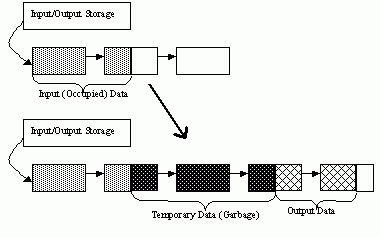
\includegraphics[width=0.5\textwidth]{pics/memstorage1.png}

That is, garbage appears in the middle of the storage. However, if
one creates a child memory storage at the beginning of processing,
writes temporary data there, and releases the child storage at the end,
no garbage will appear in the source/destination storage:

Dynamic data processing using a child storage

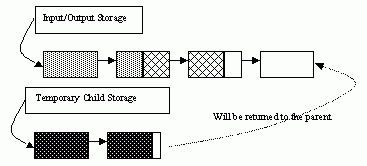
\includegraphics[width=0.5\textwidth]{pics/memstorage2.png}

\cvCPyFunc{CreateGraph}
Creates an empty graph.

\cvdefC{CvGraph* cvCreateGraph( \par int graph\_flags,\par int header\_size,\par int vtx\_size,\par int edge\_size,\par CvMemStorage* storage );}

\begin{description}
\cvarg{graph\_flags}{Type of the created graph. Usually, it is either \texttt{CV\_SEQ\_KIND\_GRAPH} for generic unoriented graphs and
\texttt{CV\_SEQ\_KIND\_GRAPH | CV\_GRAPH\_FLAG\_ORIENTED} for generic oriented graphs.}
\cvarg{header\_size}{Graph header size; may not be less than \texttt{sizeof(CvGraph)}}
\cvarg{vtx\_size}{Graph vertex size; the custom vertex structure must start with \cross{CvGraphVtx} (use \texttt{CV\_GRAPH\_VERTEX\_FIELDS()})}
\cvarg{edge\_size}{Graph edge size; the custom edge structure must start with \cross{CvGraphEdge} (use \texttt{CV\_GRAPH\_EDGE\_FIELDS()})}
\cvarg{storage}{The graph container}
\end{description}

The function creates an empty graph and returns a pointer to it.

\cvCPyFunc{CreateGraphScanner}
Creates structure for depth-first graph traversal.

\cvdefC{
CvGraphScanner*  cvCreateGraphScanner( \par CvGraph* graph,\par CvGraphVtx* vtx=NULL,\par int mask=CV\_GRAPH\_ALL\_ITEMS );
}

\begin{description}
\cvarg{graph}{Graph}
\cvarg{vtx}{Initial vertex to start from. If NULL, the traversal starts from the first vertex (a vertex with the minimal index in the sequence of vertices).}
\cvarg{mask}{Event mask indicating which events are of interest to the user (where \cvCPyCross{NextGraphItem} function returns control to the user) It can be \texttt{CV\_GRAPH\_ALL\_ITEMS} (all events are of interest) or a combination of the following flags:

\begin{description}
\cvarg{CV\_GRAPH\_VERTEX}{stop at the graph vertices visited for the first time}
\cvarg{CV\_GRAPH\_TREE\_EDGE}{stop at tree edges (\texttt{tree edge} is the edge connecting the last visited vertex and the vertex to be visited next)}
\cvarg{CV\_GRAPH\_BACK\_EDGE}{stop at back edges (\texttt{back edge} is an edge connecting the last visited vertex with some of its ancestors in the search tree)}
\cvarg{CV\_GRAPH\_FORWARD\_EDGE}{stop at forward edges (\texttt{forward edge} is an edge conecting the last visited vertex with some of its descendants in the search tree. The forward edges are only possible during oriented graph traversal)}
\cvarg{CV\_GRAPH\_CROSS\_EDGE}{stop at cross edges (\texttt{cross edge} is an edge connecting different search trees or branches of the same tree. The \texttt{cross edges} are only possible during oriented graph traversal)}
\cvarg{CV\_GRAPH\_ANY\_EDGE}{stop at any edge (\texttt{tree, back, forward}, and \texttt{cross edges})}
\cvarg{CV\_GRAPH\_NEW\_TREE}{stop in the beginning of every new search tree. When the traversal procedure visits all vertices and edges reachable from the initial vertex (the visited vertices together with tree edges make up a tree), it searches for some unvisited vertex in the graph and resumes the traversal process from that vertex. Before starting a new tree (including the very first tree when \texttt{cvNextGraphItem} is called for the first time) it generates a \texttt{CV\_GRAPH\_NEW\_TREE} event. For unoriented graphs, each search tree corresponds to a connected component of the graph.}
\cvarg{CV\_GRAPH\_BACKTRACKING}{stop at every already visited vertex during backtracking - returning to already visited vertexes of the traversal tree.}
\end{description}}
\end{description}

The function creates a structure for depth-first graph traversal/search. The initialized structure is used in the \cvCPyCross{NextGraphItem} function - the incremental traversal procedure.

\fi

\cvCPyFunc{CreateMemStorage}
Creates memory storage.

\cvdefC{CvMemStorage* cvCreateMemStorage( int blockSize=0 );}
\cvdefPy{CreateMemStorage(blockSize = 0) -> memstorage}

\begin{description}
\cvarg{blockSize}{Size of the storage blocks in bytes. If it is 0, the block size is set to a default value - currently it is  about 64K.}
\end{description}

The function creates an empty memory storage. See \cross{CvMemStorage} description.

\ifC

\cvCPyFunc{CreateSeq}
Creates a sequence.

\cvdefC{CvSeq* cvCreateSeq( \par int seqFlags,\par int headerSize,\par int elemSize,\par CvMemStorage* storage);}

\begin{description}
\cvarg{seqFlags}{Flags of the created sequence. If the sequence is not passed to any function working with a specific type of sequences, the sequence value may be set to 0, otherwise the appropriate type must be selected from the list of predefined sequence types.}
\cvarg{headerSize}{Size of the sequence header; must be greater than or equal to \texttt{sizeof(CvSeq)}. If a specific type or its extension is indicated, this type must fit the base type header.}
\cvarg{elemSize}{Size of the sequence elements in bytes. The size must be consistent with the sequence type. For example, for a sequence of points to be created, the element type \newline \texttt{CV\_SEQ\_ELTYPE\_POINT} should be specified and the parameter \texttt{elemSize} must be equal to \texttt{sizeof(CvPoint)}.}
\cvarg{storage}{Sequence location}
\end{description}

The function creates a sequence and returns
the pointer to it. The function allocates the sequence header in
the storage block as one continuous chunk and sets the structure
fields \texttt{flags}, \texttt{elemSize}, \texttt{headerSize}, and
\texttt{storage} to passed values, sets \texttt{delta\_elems} to the
default value (that may be reassigned using the \cvCPyCross{SetSeqBlockSize}
function), and clears other header fields, including the space following
the first \texttt{sizeof(CvSeq)} bytes.

\cvCPyFunc{CreateSet}
Creates an empty set.

\cvdefC{CvSet* cvCreateSet( \par int set\_flags,\par int header\_size,\par int elem\_size,\par CvMemStorage* storage );}

\begin{description}
\cvarg{set\_flags}{Type of the created set}
\cvarg{header\_size}{Set header size; may not be less than \texttt{sizeof(CvSet)}}
\cvarg{elem\_size}{Set element size; may not be less than \cross{CvSetElem}}
\cvarg{storage}{Container for the set}
\end{description}

The function creates an empty set with a specified header size and element size, and returns the pointer to the set. This function is just a thin layer on top of \cvCPyCross{CreateSeq}.

\cvCPyFunc{CvtSeqToArray}
Copies a sequence to one continuous block of memory.

\cvdefC{void* cvCvtSeqToArray( \par const CvSeq* seq,\par void* elements,\par CvSlice slice=CV\_WHOLE\_SEQ );}

\begin{description}
\cvarg{seq}{Sequence}
\cvarg{elements}{Pointer to the destination array that must be large enough. It should be a pointer to data, not a matrix header.}
\cvarg{slice}{The sequence portion to copy to the array}
\end{description}

The function copies the entire sequence or subsequence to the specified buffer and returns the pointer to the buffer.

\cvCPyFunc{EndWriteSeq}
Finishes the process of writing a sequence.

\cvdefC{CvSeq* cvEndWriteSeq( CvSeqWriter* writer );}

\begin{description}
\cvarg{writer}{Writer state}
\end{description}


The function finishes the writing process and
returns the pointer to the written sequence. The function also truncates
the last incomplete sequence block to return the remaining part of the
block to memory storage. After that, the sequence can be read and
modified safely. See \cvCPyCross{cvStartWriteSeq} and \cvCPyCross{cvStartAppendToSeq}

\cvCPyFunc{FindGraphEdge}
Finds an edge in a graph.

\cvdefC{
CvGraphEdge* cvFindGraphEdge( const CvGraph* graph, int start\_idx, int end\_idx );
}

\begin{lstlisting}

#define cvGraphFindEdge cvFindGraphEdge

\end{lstlisting}

\begin{description}
\cvarg{graph}{Graph}
\cvarg{start\_idx}{Index of the starting vertex of the edge}
\cvarg{end\_idx}{Index of the ending vertex of the edge. For an unoriented graph, the order of the vertex parameters does not matter.}
\end{description}

The function finds the graph edge connecting two specified vertices and returns a pointer to it or NULL if the edge does not exist.

\cvCPyFunc{FindGraphEdgeByPtr}
Finds an edge in a graph by using its pointer.

\cvdefC{
CvGraphEdge* cvFindGraphEdgeByPtr( \par const CvGraph* graph,\par const CvGraphVtx* startVtx,\par const CvGraphVtx* endVtx );
}

\begin{lstlisting}
#define cvGraphFindEdgeByPtr cvFindGraphEdgeByPtr
\end{lstlisting}

\begin{description}
\cvarg{graph}{Graph}
\cvarg{startVtx}{Pointer to the starting vertex of the edge}
\cvarg{endVtx}{Pointer to the ending vertex of the edge. For an unoriented graph, the order of the vertex parameters does not matter.}
\end{description}

The function finds the graph edge connecting two specified vertices and returns pointer to it or NULL if the edge does not exists.

\cvCPyFunc{FlushSeqWriter}
Updates sequence headers from the writer.

\cvdefC{void cvFlushSeqWriter( CvSeqWriter* writer );}

\begin{description}
\cvarg{writer}{Writer state}
\end{description}

The function is intended to enable the user to
read sequence elements, whenever required, during the writing process,
e.g., in order to check specific conditions. The function updates the
sequence headers to make reading from the sequence possible. The writer
is not closed, however, so that the writing process can be continued at
any time. If an algorithm requires frequent flushes, consider using
\cvCPyCross{SeqPush} instead.

\cvCPyFunc{GetGraphVtx}
Finds a graph vertex by using its index.

\cvdefC{CvGraphVtx* cvGetGraphVtx( \par CvGraph* graph,\par int vtx\_idx );}

\begin{description}
\cvarg{graph}{Graph}
\cvarg{vtx\_idx}{Index of the vertex}
\end{description}


The function finds the graph vertex by using its index and returns the pointer to it or NULL if the vertex does not belong to the graph.


\cvCPyFunc{GetSeqElem}
Returns a pointer to a sequence element according to its index.

\cvdefC{char* cvGetSeqElem( const CvSeq* seq, int index );}

\begin{lstlisting}
#define CV_GET_SEQ_ELEM( TYPE, seq, index )  (TYPE*)cvGetSeqElem( (CvSeq*)(seq), (index) )
\end{lstlisting}

\begin{description}
\cvarg{seq}{Sequence}
\cvarg{index}{Index of element}
\end{description}

The function finds the element with the given
index in the sequence and returns the pointer to it. If the element
is not found, the function returns 0. The function supports negative
indices, where -1 stands for the last sequence element, -2 stands for
the one before last, etc. If the sequence is most likely to consist of
a single sequence block or the desired element is likely to be located
in the first block, then the macro
\texttt{CV\_GET\_SEQ\_ELEM( elemType, seq, index )}
should be used, where the parameter \texttt{elemType} is the
type of sequence elements ( \cross{CvPoint} for example), the parameter
\texttt{seq} is a sequence, and the parameter \texttt{index} is the index
of the desired element. The macro checks first whether the desired element
belongs to the first block of the sequence and returns it if it does;
otherwise the macro calls the main function \texttt{GetSeqElem}. Negative
indices always cause the \cvCPyCross{GetSeqElem} call. The function has O(1)
time complexity assuming that the number of blocks is much smaller than the
number of elements.

\cvCPyFunc{GetSeqReaderPos}
Returns the current reader position.

\cvdefC{int cvGetSeqReaderPos( CvSeqReader* reader );}

\begin{description}
\cvarg{reader}{Reader state}
\end{description}


The function returns the current reader position (within 0 ... \texttt{reader->seq->total} - 1).

\cvCPyFunc{GetSetElem}
Finds a set element by its index.

\cvdefC{CvSetElem* cvGetSetElem( \par const CvSet* setHeader,\par int index );}

\begin{description}
\cvarg{setHeader}{Set}
\cvarg{index}{Index of the set element within a sequence}
\end{description}

The function finds a set element by its index. The function returns the pointer to it or 0 if the index is invalid or the corresponding node is free. The function supports negative indices as it uses \cvCPyCross{GetSeqElem} to locate the node.

\cvCPyFunc{GraphAddEdge}
Adds an edge to a graph.

\cvdefC{int cvGraphAddEdge( \par CvGraph* graph,\par int start\_idx,\par int end\_idx,\par const CvGraphEdge* edge=NULL,\par CvGraphEdge** inserted\_edge=NULL );
}

\begin{description}
\cvarg{graph}{Graph}
\cvarg{start\_idx}{Index of the starting vertex of the edge}
\cvarg{end\_idx}{Index of the ending vertex of the edge. For an unoriented graph, the order of the vertex parameters does not matter.}
\cvarg{edge}{Optional input parameter, initialization data for the edge}
\cvarg{inserted\_edge}{Optional output parameter to contain the address of the inserted edge}
\end{description}


The function connects two specified vertices. The function returns 1 if the edge has been added successfully, 0 if the edge connecting the two vertices exists already and -1 if either of the vertices was not found, the starting and the ending vertex are the same, or there is some other critical situation. In the latter case (i.e., when the result is negative), the function also reports an error by default.

\cvCPyFunc{GraphAddEdgeByPtr}
Adds an edge to a graph by using its pointer.

\cvdefC{int cvGraphAddEdgeByPtr( \par CvGraph* graph,\par CvGraphVtx* start\_vtx,\par CvGraphVtx* end\_vtx,\par const CvGraphEdge* edge=NULL,\par CvGraphEdge** inserted\_edge=NULL );}

\begin{description}
\cvarg{graph}{Graph}
\cvarg{start\_vtx}{Pointer to the starting vertex of the edge}
\cvarg{end\_vtx}{Pointer to the ending vertex of the edge. For an unoriented graph, the order of the vertex parameters does not matter.}
\cvarg{edge}{Optional input parameter, initialization data for the edge}
\cvarg{inserted\_edge}{Optional output parameter to contain the address of the inserted edge within the edge set}
\end{description}

The function connects two specified vertices. The
function returns 1 if the edge has been added successfully, 0 if the
edge connecting the two vertices exists already, and -1 if either of the
vertices was not found, the starting and the ending vertex are the same
or there is some other critical situation. In the latter case (i.e., when
the result is negative), the function also reports an error by default.

\cvCPyFunc{GraphAddVtx}
Adds a vertex to a graph.

\cvdefC{
int cvGraphAddVtx( \par CvGraph* graph,\par const CvGraphVtx* vtx=NULL,\par CvGraphVtx** inserted\_vtx=NULL );}

\begin{description}
\cvarg{graph}{Graph}
\cvarg{vtx}{Optional input argument used to initialize the added vertex (only user-defined fields beyond \texttt{sizeof(CvGraphVtx)} are copied)}
\cvarg{inserted\_vertex}{Optional output argument. If not \texttt{NULL}, the address of the new vertex is written here.}
\end{description}

The function adds a vertex to the graph and returns the vertex index.

\cvCPyFunc{GraphEdgeIdx}
Returns the index of a graph edge.

\cvdefC{
int cvGraphEdgeIdx( \par CvGraph* graph,\par CvGraphEdge* edge );
}

\begin{description}
\cvarg{graph}{Graph}
\cvarg{edge}{Pointer to the graph edge}
\end{description}

The function returns the index of a graph edge.

\cvCPyFunc{GraphRemoveEdge}
Removes an edge from a graph.

\cvdefC{void cvGraphRemoveEdge( \par CvGraph* graph,\par int start\_idx,\par int end\_idx );}

\begin{description}
\cvarg{graph}{Graph}
\cvarg{start\_idx}{Index of the starting vertex of the edge}
\cvarg{end\_idx}{Index of the ending vertex of the edge. For an unoriented graph, the order of the vertex parameters does not matter.}
\end{description}

The function removes the edge connecting two specified vertices. If the vertices are not connected [in that order], the function does nothing.

\cvCPyFunc{GraphRemoveEdgeByPtr}

Removes an edge from a graph by using its pointer.

\cvdefC{void cvGraphRemoveEdgeByPtr( \par CvGraph* graph,\par CvGraphVtx* start\_vtx,\par CvGraphVtx* end\_vtx );}

\begin{description}
\cvarg{graph}{Graph}
\cvarg{start\_vtx}{Pointer to the starting vertex of the edge}
\cvarg{end\_vtx}{Pointer to the ending vertex of the edge. For an unoriented graph, the order of the vertex parameters does not matter.}
\end{description}

The function removes the edge connecting two specified vertices. If the vertices are not connected [in that order], the function does nothing.

\cvCPyFunc{GraphRemoveVtx}
Removes a vertex from a graph.

\cvdefC{int cvGraphRemoveVtx( \par CvGraph* graph,\par int index );}

\begin{description}
\cvarg{graph}{Graph}
\cvarg{vtx\_idx}{Index of the removed vertex}
\end{description}

The function removes a vertex from a graph
together with all the edges incident to it. The function reports an error
if the input vertex does not belong to the graph. The return value is the
number of edges deleted, or -1 if the vertex does not belong to the graph.

\cvCPyFunc{GraphRemoveVtxByPtr}
Removes a vertex from a graph by using its pointer.

\cvdefC{int cvGraphRemoveVtxByPtr( \par CvGraph* graph,\par CvGraphVtx* vtx );}

\begin{description}
\cvarg{graph}{Graph}
\cvarg{vtx}{Pointer to the removed vertex}
\end{description}


The function removes a vertex from the graph by using its pointer together with all the edges incident to it. The function reports an error if the vertex does not belong to the graph. The return value is the number of edges deleted, or -1 if the vertex does not belong to the graph.

\cvCPyFunc{GraphVtxDegree}
Counts the number of edges indicent to the vertex.

\cvdefC{
int cvGraphVtxDegree( const CvGraph* graph, int vtxIdx );
}

\begin{description}
\cvarg{graph}{Graph}
\cvarg{vtxIdx}{Index of the graph vertex}
\end{description}

The function returns the number of edges incident to the specified vertex, both incoming and outgoing. To count the edges, the following code is used:

\begin{lstlisting}
CvGraphEdge* edge = vertex->first; int count = 0;
while( edge )
{
    edge = CV_NEXT_GRAPH_EDGE( edge, vertex );
    count++;
}
\end{lstlisting}

The macro \texttt{CV\_NEXT\_GRAPH\_EDGE( edge, vertex )} returns the edge incident to \texttt{vertex} that follows after \texttt{edge}.

\cvCPyFunc{GraphVtxDegreeByPtr}
Finds an edge in a graph.

\cvdefC{
int cvGraphVtxDegreeByPtr( \par const CvGraph* graph,\par const CvGraphVtx* vtx );
}

\begin{description}
\cvarg{graph}{Graph}
\cvarg{vtx}{Pointer to the graph vertex}
\end{description}

The function returns the number of edges incident to the specified vertex, both incoming and outcoming.


\cvCPyFunc{GraphVtxIdx}
Returns the index of a graph vertex.

\cvdefC{int cvGraphVtxIdx( \par CvGraph* graph,\par CvGraphVtx* vtx );}

\begin{description}
\cvarg{graph}{Graph}
\cvarg{vtx}{Pointer to the graph vertex}
\end{description}

The function returns the index of a graph vertex.

\cvCPyFunc{InitTreeNodeIterator}

Initializes the tree node iterator.

\cvdefC{

void cvInitTreeNodeIterator( \par CvTreeNodeIterator* tree\_iterator,\par const void* first,\par int max\_level );

}

\begin{description}
\cvarg{tree\_iterator}{Tree iterator initialized by the function}
\cvarg{first}{The initial node to start traversing from}
\cvarg{max\_level}{The maximal level of the tree (\texttt{first} node assumed to be at the first level) to traverse up to. For example, 1 means that only nodes at the same level as \texttt{first} should be visited, 2 means that the nodes on the same level as \texttt{first} and their direct children should be visited, and so forth.}
\end{description}

The function initializes the tree iterator. The tree is traversed in depth-first order.

\cvCPyFunc{InsertNodeIntoTree}

Adds a new node to a tree.

\cvdefC{void cvInsertNodeIntoTree( \par void* node,\par void* parent,\par void* frame );}

\begin{description}
\cvarg{node}{The inserted node}
\cvarg{parent}{The parent node that is already in the tree}
\cvarg{frame}{The top level node. If \texttt{parent} and \texttt{frame} are the same, the \texttt{v\_prev} field of \texttt{node} is set to NULL rather than \texttt{parent}.}
\end{description}

The function adds another node into tree. The function does not allocate any memory, it can only modify links of the tree nodes.

\cvCPyFunc{MakeSeqHeaderForArray}
Constructs a sequence header for an array.

\cvdefC{CvSeq* cvMakeSeqHeaderForArray( \par int seq\_type,\par int header\_size,\par int elem\_size,\par void* elements,\par int total,\par CvSeq* seq,\par CvSeqBlock* block );}

\begin{description}
\cvarg{seq\_type}{Type of the created sequence}
\cvarg{header\_size}{Size of the header of the sequence. Parameter sequence must point to the structure of that size or greater}
\cvarg{elem\_size}{Size of the sequence elements}
\cvarg{elements}{Elements that will form a sequence}
\cvarg{total}{Total number of elements in the sequence. The number of array elements must be equal to the value of this parameter.}
\cvarg{seq}{Pointer to the local variable that is used as the sequence header}
\cvarg{block}{Pointer to the local variable that is the header of the single sequence block}
\end{description}

The function initializes a sequence
header for an array. The sequence header as well as the sequence block are
allocated by the user (for example, on stack). No data is copied by the
function. The resultant sequence will consists of a single block and
have NULL storage pointer; thus, it is possible to read its elements,
but the attempts to add elements to the sequence will raise an error in
most cases.

\cvCPyFunc{MemStorageAlloc}
Allocates a memory buffer in a storage block.

\cvdefC{void* cvMemStorageAlloc( \par CvMemStorage* storage,\par size\_t size );}

\begin{description}
\cvarg{storage}{Memory storage}
\cvarg{size}{Buffer size}
\end{description}

The function allocates a memory buffer in
a storage block. The buffer size must not exceed the storage block size,
otherwise a runtime error is raised. The buffer address is aligned by
\texttt{CV\_STRUCT\_ALIGN=sizeof(double)} (for the moment) bytes.

\cvCPyFunc{MemStorageAllocString}
Allocates a text string in a storage block.

\cvdefC{CvString cvMemStorageAllocString(CvMemStorage* storage, const char* ptr, int len=-1);}

\begin{lstlisting}
typedef struct CvString
{
    int len;
    char* ptr;
}
CvString;
\end{lstlisting}

\begin{description}
\cvarg{storage}{Memory storage}
\cvarg{ptr}{The string}
\cvarg{len}{Length of the string (not counting the ending \texttt{NUL}) . If the parameter is negative, the function computes the length.}
\end{description}

The function creates copy of the string
in memory storage. It returns the structure that contains user-passed
or computed length of the string and pointer to the copied string.

\cvCPyFunc{NextGraphItem}
Executes one or more steps of the graph traversal procedure.

\cvdefC{
int cvNextGraphItem( CvGraphScanner* scanner );
}

\begin{description}
\cvarg{scanner}{Graph traversal state. It is updated by this function.}
\end{description}

The function traverses through the graph
until an event of interest to the user (that is, an event, specified
in the \texttt{mask} in the \cvCPyCross{CreateGraphScanner} call) is met or the
traversal is completed. In the first case, it returns one of the events
listed in the description of the \texttt{mask} parameter above and with
the next call it resumes the traversal. In the latter case, it returns
\texttt{CV\_GRAPH\_OVER} (-1). When the event is \texttt{CV\_GRAPH\_VERTEX},
\texttt{CV\_GRAPH\_BACKTRACKING}, or \texttt{CV\_GRAPH\_NEW\_TREE},
the currently observed vertex is stored in \texttt{scanner-$>$vtx}. And if the
event is edge-related, the edge itself is stored at \texttt{scanner-$>$edge},
the previously visited vertex - at \texttt{scanner-$>$vtx} and the other ending
vertex of the edge - at \texttt{scanner-$>$dst}.

\cvCPyFunc{NextTreeNode}

Returns the currently observed node and moves the iterator toward the next node.

\cvdefC{

void* cvNextTreeNode( CvTreeNodeIterator* tree\_iterator );

}

\begin{description}
\cvarg{tree\_iterator}{Tree iterator initialized by the function}
\end{description}


The function returns the currently observed node and then updates the
iterator - moving it toward the next node. In other words, the function
behavior is similar to the \texttt{*p++} expression on a typical C
pointer or C++ collection iterator. The function returns NULL if there
are no more nodes.


\cvCPyFunc{PrevTreeNode}

Returns the currently observed node and moves the iterator toward the previous node.

\cvdefC{

void* cvPrevTreeNode( CvTreeNodeIterator* tree\_iterator );

}

\begin{description}
\cvarg{tree\_iterator}{Tree iterator initialized by the function}
\end{description}


The function returns the currently observed node and then updates
the iterator - moving it toward the previous node. In other words,
the function behavior is similar to the \texttt{*p--} expression on a
typical C pointer or C++ collection iterator. The function returns NULL
if there are no more nodes.


\cvCPyFunc{ReleaseGraphScanner}
Completes the graph traversal procedure.

\cvdefC{
void cvReleaseGraphScanner( CvGraphScanner** scanner );
}

\begin{description}
\cvarg{scanner}{Double pointer to graph traverser}
\end{description}


The function completes the graph traversal procedure and releases the traverser state.



\cvCPyFunc{ReleaseMemStorage}
Releases memory storage.

\cvdefC{void cvReleaseMemStorage( CvMemStorage** storage );}

\begin{description}
\cvarg{storage}{Pointer to the released storage}
\end{description}

The function deallocates all storage memory
blocks or returns them to the parent, if any. Then it deallocates the
storage header and clears the pointer to the storage. All child storage 
associated with a given parent storage block must be released before the 
parent storage block is released.

\cvCPyFunc{RestoreMemStoragePos}
Restores memory storage position.

\cvdefC{void cvRestoreMemStoragePos(\par CvMemStorage* storage,\par CvMemStoragePos* pos);}

\begin{description}
\cvarg{storage}{Memory storage}
\cvarg{pos}{New storage top position}
\end{description}

The function restores the position of the storage top from the parameter \texttt{pos}. This function and the function \texttt{cvClearMemStorage} are the only methods to release memory occupied in memory blocks. Note again that there is no way to free memory in the middle of an occupied portion of a storage block.


\cvCPyFunc{SaveMemStoragePos}
Saves memory storage position.

\cvdefC{void cvSaveMemStoragePos(\par const CvMemStorage* storage,\par CvMemStoragePos* pos);}

\begin{description}
\cvarg{storage}{Memory storage}
\cvarg{pos}{The output position of the storage top}
\end{description}

The function saves the current position
of the storage top to the parameter \texttt{pos}. The function
\texttt{cvRestoreMemStoragePos} can further retrieve this position.

\cvCPyFunc{SeqElemIdx}
Returns the index of a specific sequence element.

\cvdefC{int cvSeqElemIdx( \par const CvSeq* seq,\par const void* element,\par CvSeqBlock** block=NULL );}

\begin{description}
\cvarg{seq}{Sequence}
\cvarg{element}{Pointer to the element within the sequence}
\cvarg{block}{Optional argument. If the pointer is not \texttt{NULL}, the address of the sequence block that contains the element is stored in this location.}
\end{description}

The function returns the index of a sequence element or a negative number if the element is not found.

\cvCPyFunc{SeqInsert}
Inserts an element in the middle of a sequence.

\cvdefC{char* cvSeqInsert( \par CvSeq* seq,\par int beforeIndex,\par void* element=NULL );}

\begin{description}
\cvarg{seq}{Sequence}
\cvarg{beforeIndex}{Index before which the element is inserted. Inserting before 0 (the minimal allowed value of the parameter) is equal to \cvCPyCross{SeqPushFront} and inserting before \texttt{seq->total} (the maximal allowed value of the parameter) is equal to \cvCPyCross{SeqPush}.}
\cvarg{element}{Inserted element} 
\end{description}

The function shifts the sequence elements from the inserted position to the nearest end of the sequence and copies the \texttt{element} content there if the pointer is not NULL. The function returns a pointer to the inserted element.


\cvCPyFunc{SeqInsertSlice}
Inserts an array in the middle of a sequence.

\cvdefC{void cvSeqInsertSlice( \par CvSeq* seq,\par int beforeIndex,\par const CvArr* fromArr );}

\begin{description}
\cvarg{seq}{Sequence}
\cvarg{slice}{The part of the sequence to remove}
\cvarg{fromArr}{The array to take elements from}
\end{description}


The function inserts all \texttt{fromArr}
array elements at the specified position of the sequence. The array
\texttt{fromArr} can be a matrix or another sequence.

\fi

\cvCPyFunc{SeqInvert}
Reverses the order of sequence elements.

\cvdefC{void cvSeqInvert( CvSeq* seq );}
\cvdefPy{SeqInvert(seq)-> None}

\begin{description}
\cvarg{seq}{Sequence}
\end{description}


The function reverses the sequence in-place - makes the first element go last, the last element go first and so forth.

\ifC

\cvCPyFunc{SeqPop}
Removes an element from the end of a sequence.

\cvdefC{void cvSeqPop( \par CvSeq* seq,\par void* element=NULL );}

\begin{description}
\cvarg{seq}{Sequence}
\cvarg{element}{Optional parameter . If the pointer is not zero, the function copies the removed element to this location.}
\end{description}

The function removes an element from a sequence. The function reports an error if the sequence is already empty. The function has O(1) complexity.

\cvCPyFunc{SeqPopFront}
Removes an element from the beginning of a sequence.

\cvdefC{void cvSeqPopFront( \par \par CvSeq* seq,\par\par void* element=NULL );}

\begin{description}
\cvarg{seq}{Sequence}
\cvarg{element}{Optional parameter. If the pointer is not zero, the function copies the removed element to this location.}
\end{description}

The function removes an element from the beginning of a sequence. The function reports an error if the sequence is already empty. The function has O(1) complexity.

\cvCPyFunc{SeqPopMulti}
Removes several elements from either end of a sequence.

\cvdefC{void cvSeqPopMulti( \par CvSeq* seq,\par void* elements,\par int count,\par int in\_front=0 );}

\begin{description}
\cvarg{seq}{Sequence}
\cvarg{elements}{Removed elements}
\cvarg{count}{Number of elements to pop}
\cvarg{in\_front}{The flags specifying which end of the modified sequence.
\begin{description}
\cvarg{CV\_BACK}{the elements are added to the end of the sequence}
\cvarg{CV\_FRONT}{the elements are added to the beginning of the sequence}
\end{description}}
\end{description}

The function removes several elements from either end of the sequence. If the number of the elements to be removed exceeds the total number of elements in the sequence, the function removes as many elements as possible.

\cvCPyFunc{SeqPush}
Adds an element to the end of a sequence.

\cvdefC{char* cvSeqPush( \par CvSeq* seq,\par void* element=NULL );}

\begin{description}
\cvarg{seq}{Sequence}
\cvarg{element}{Added element}
\end{description}

The function adds an element to the end of a sequence and returns a pointer to the allocated element. If the input \texttt{element} is NULL, the function simply allocates a space for one more element.

The following code demonstrates how to create a new sequence using this function:

\begin{lstlisting}
CvMemStorage* storage = cvCreateMemStorage(0);
CvSeq* seq = cvCreateSeq( CV_32SC1, /* sequence of integer elements */
                          sizeof(CvSeq), /* header size - no extra fields */
                          sizeof(int), /* element size */
                          storage /* the container storage */ );
int i;
for( i = 0; i < 100; i++ )
{
    int* added = (int*)cvSeqPush( seq, &i );
    printf( "%d is added\n", *added );
}

...
/* release memory storage in the end */
cvReleaseMemStorage( &storage );
\end{lstlisting}

The function has O(1) complexity, but there is a faster method for writing large sequences (see \cvCPyCross{StartWriteSeq} and related functions).


\cvCPyFunc{SeqPushFront}
Adds an element to the beginning of a sequence.

\cvdefC{char* cvSeqPushFront( CvSeq* seq, void* element=NULL );}

\begin{description}
\cvarg{seq}{Sequence}
\cvarg{element}{Added element}
\end{description}

The function is similar to \cvCPyCross{SeqPush} but it adds the new element to the beginning of the sequence. The function has O(1) complexity.

\cvCPyFunc{SeqPushMulti}
Pushes several elements to either end of a sequence.

\cvdefC{void cvSeqPushMulti( \par CvSeq* seq,\par void* elements,\par int count,\par int in\_front=0 );}

\begin{description}
\cvarg{seq}{Sequence}
\cvarg{elements}{Added elements}
\cvarg{count}{Number of elements to push}
\cvarg{in\_front}{The flags specifying which end of the modified sequence.
\begin{description}
\cvarg{CV\_BACK}{the elements are added to the end of the sequence}
\cvarg{CV\_FRONT}{the elements are added to the beginning of the sequence}
\end{description}}
\end{description}

The function adds several elements to either
end of a sequence. The elements are added to the sequence in the same
order as they are arranged in the input array but they can fall into
different sequence blocks.

\fi

\cvCPyFunc{SeqRemove}
Removes an element from the middle of a sequence.

\cvdefC{void cvSeqRemove( \par CvSeq* seq,\par int index );}
\cvdefPy{SeqRemove(seq,index)-> None}

\begin{description}
\cvarg{seq}{Sequence}
\cvarg{index}{Index of removed element}
\end{description}

The function removes elements with the given
index. If the index is out of range the function reports an error. An
attempt to remove an element from an empty sequence is a special
case of this situation. The function removes an element by shifting
the sequence elements between the nearest end of the sequence and the
\texttt{index}-th position, not counting the latter.


\cvCPyFunc{SeqRemoveSlice}
Removes a sequence slice.

\cvdefC{void cvSeqRemoveSlice( CvSeq* seq, CvSlice slice );}
\cvdefPy{SeqRemoveSlice(seq,slice)-> None}

\begin{description}
\cvarg{seq}{Sequence}
\cvarg{slice}{The part of the sequence to remove}
\end{description}

The function removes a slice from the sequence.

\ifC

\cvCPyFunc{SeqSearch}
Searches for an element in a sequence.

\cvdefC{
char* cvSeqSearch( CvSeq* seq, const void* elem, CvCmpFunc func,
                   int is\_sorted, int* elem\_idx, void* userdata=NULL );
}

\begin{description}
\cvarg{seq}{The sequence}
\cvarg{elem}{The element to look for}
\cvarg{func}{The comparison function that returns negative, zero or positive value depending on the relationships among the elements (see also \cvCPyCross{SeqSort})}
\cvarg{is\_sorted}{Whether the sequence is sorted or not}
\cvarg{elem\_idx}{Output parameter; index of the found element}
\cvarg{userdata}{The user parameter passed to the compasion function; helps to avoid global variables in some cases}
\end{description}

\begin{lstlisting}
/* a < b ? -1 : a > b ? 1 : 0 */
typedef int (CV_CDECL* CvCmpFunc)(const void* a, const void* b, void* userdata);
\end{lstlisting}

The function searches for the element in the sequence. If
the sequence is sorted, a binary O(log(N)) search is used; otherwise, a
simple linear search is used. If the element is not found, the function
returns a NULL pointer and the index is set to the number of sequence
elements if a linear search is used, or to the smallest index
\texttt{i, seq(i)>elem}.

\cvCPyFunc{SeqSlice}
Makes a separate header for a sequence slice.

\cvdefC{CvSeq* cvSeqSlice( \par const CvSeq* seq,\par CvSlice slice,\par CvMemStorage* storage=NULL,\par int copy\_data=0 );}

\begin{description}
\cvarg{seq}{Sequence}
\cvarg{slice}{The part of the sequence to be extracted}
\cvarg{storage}{The destination storage block to hold the new sequence header and the copied data, if any. If it is NULL, the function uses the storage block containing the input sequence.}
\cvarg{copy\_data}{The flag that indicates whether to copy the elements of the extracted slice (\texttt{copy\_data!=0}) or not (\texttt{copy\_data=0})}
\end{description}

The function creates a sequence that represents the specified slice of the input sequence. The new sequence either shares the elements with the original sequence or has its own copy of the elements. So if one needs to process a part of sequence but the processing function does not have a slice parameter, the required sub-sequence may be extracted using this function.

\cvCPyFunc{SeqSort}
Sorts sequence element using the specified comparison function.

\cvdefC{void cvSeqSort( CvSeq* seq, CvCmpFunc func, void* userdata=NULL );}

\begin{lstlisting}
/* a < b ? -1 : a > b ? 1 : 0 */
typedef int (CV_CDECL* CvCmpFunc)(const void* a, const void* b, void* userdata);
\end{lstlisting}

\begin{description}
\cvarg{seq}{The sequence to sort}
\cvarg{func}{The comparison function that returns a negative, zero, or positive value depending on the relationships among the elements (see the above declaration and the example below) - a similar function is used by \texttt{qsort} from C runline except that in the latter, \texttt{userdata} is not used}
\cvarg{userdata}{The user parameter passed to the compasion function; helps to avoid global variables in some cases}
\end{description}

The function sorts the sequence in-place using the specified criteria. Below is an example of using this function:

\begin{lstlisting}
/* Sort 2d points in top-to-bottom left-to-right order */
static int cmp_func( const void* _a, const void* _b, void* userdata )
{
    CvPoint* a = (CvPoint*)_a;
    CvPoint* b = (CvPoint*)_b;
    int y_diff = a->y - b->y;
    int x_diff = a->x - b->x;
    return y_diff ? y_diff : x_diff;
}

...

CvMemStorage* storage = cvCreateMemStorage(0);
CvSeq* seq = cvCreateSeq( CV_32SC2, sizeof(CvSeq), sizeof(CvPoint), storage );
int i;

for( i = 0; i < 10; i++ )
{
    CvPoint pt;
    pt.x = rand() % 1000;
    pt.y = rand() % 1000;
    cvSeqPush( seq, &pt );
}

cvSeqSort( seq, cmp_func, 0 /* userdata is not used here */ );

/* print out the sorted sequence */
for( i = 0; i < seq->total; i++ )
{
    CvPoint* pt = (CvPoint*)cvSeqElem( seq, i );
    printf( "(%d,%d)\n", pt->x, pt->y );
}

cvReleaseMemStorage( &storage );
\end{lstlisting}


\cvCPyFunc{SetAdd}
Occupies a node in the set.

\cvdefC{int cvSetAdd( \par CvSet* setHeader,\par CvSetElem* elem=NULL,\par CvSetElem** inserted\_elem=NULL );}

\begin{description}
\cvarg{setHeader}{Set}
\cvarg{elem}{Optional input argument, an inserted element. If not NULL, the function copies the data to the allocated node (the MSB of the first integer field is cleared after copying).}
\cvarg{inserted\_elem}{Optional output argument; the pointer to the allocated cell}
\end{description}

The function allocates a new node, optionally copies
input element data to it, and returns the pointer and the index to the
node. The index value is taken from the lower bits of the \texttt{flags}
field of the node. The function has O(1) complexity; however, there exists
a faster function for allocating set nodes (see \cvCPyCross{SetNew}).

\cvCPyFunc{SetNew}
Adds an element to a set (fast variant).

\cvdefC{CvSetElem* cvSetNew( CvSet* setHeader );}

\begin{description}
\cvarg{setHeader}{Set}
\end{description}

The function is an inline lightweight variant of \cvCPyCross{SetAdd}. It occupies a new node and returns a pointer to it rather than an index.


\cvCPyFunc{SetRemove}
Removes an element from a set.

\cvdefC{void cvSetRemove( \par CvSet* setHeader,\par int index );}

\begin{description}
\cvarg{setHeader}{Set}
\cvarg{index}{Index of the removed element}
\end{description}

The function removes an element with a specified
index from the set. If the node at the specified location is not occupied,
the function does nothing. The function has O(1) complexity; however,
\cvCPyCross{SetRemoveByPtr} provides a quicker way to remove a set element
if it is located already.

\cvCPyFunc{SetRemoveByPtr}
Removes a set element based on its pointer.

\cvdefC{void cvSetRemoveByPtr( \par CvSet* setHeader,\par void* elem );}

\begin{description}
\cvarg{setHeader}{Set}
\cvarg{elem}{Removed element}
\end{description}

The function is an inline lightweight variant of \cvCPyCross{SetRemove} that requires an element pointer. The function does not check whether the node is occupied or not - the user should take care of that.


\cvCPyFunc{SetSeqBlockSize}
Sets up sequence block size.

\cvdefC{void cvSetSeqBlockSize( \par CvSeq* seq,\par int deltaElems );}

\begin{description}
\cvarg{seq}{Sequence}
\cvarg{deltaElems}{Desirable sequence block size for elements}
\end{description}

The function affects memory allocation
granularity. When the free space in the sequence buffers has run out,
the function allocates the space for \texttt{deltaElems} sequence
elements. If this block immediately follows the one previously allocated,
the two blocks are concatenated; otherwise, a new sequence block is
created. Therefore, the bigger the parameter is, the lower the possible
sequence fragmentation, but the more space in the storage block is wasted. When
the sequence is created, the parameter \texttt{deltaElems} is set to
the default value of about 1K. The function can be called any time after
the sequence is created and affects future allocations. The function
can modify the passed value of the parameter to meet memory storage
constraints.

\cvCPyFunc{SetSeqReaderPos}
Moves the reader to the specified position.

\cvdefC{void cvSetSeqReaderPos( \par CvSeqReader* reader,\par int index,\par int is\_relative=0 );}

\begin{description}
\cvarg{reader}{Reader state}
\cvarg{index}{The destination position. If the positioning mode is used (see the next parameter), the actual position will be \texttt{index} mod \texttt{reader->seq->total}.}
\cvarg{is\_relative}{If it is not zero, then \texttt{index} is a relative to the current position}
\end{description}

The function moves the read position to an absolute position or relative to the current position.


\cvCPyFunc{StartAppendToSeq}
Initializes the process of writing data to a sequence.

\cvdefC{void cvStartAppendToSeq( \par CvSeq* seq,\par CvSeqWriter* writer );}

\begin{description}
\cvarg{seq}{Pointer to the sequence}
\cvarg{writer}{Writer state; initialized by the function}
\end{description}

The function initializes the process of
writing data to a sequence. Written elements are added to the end of the
sequence by using the
\texttt{CV\_WRITE\_SEQ\_ELEM( written\_elem, writer )}
macro. Note
that during the writing process, other operations on the sequence may
yield an incorrect result or even corrupt the sequence (see description of
\cvCPyCross{FlushSeqWriter}, which helps to avoid some of these problems).

\cvCPyFunc{StartReadSeq}
Initializes the process of sequential reading from a sequence.

\cvdefC{void cvStartReadSeq( \par const CvSeq* seq,\par CvSeqReader* reader,\par int reverse=0 );}

\begin{description}
\cvarg{seq}{Sequence}
\cvarg{reader}{Reader state; initialized by the function}
\cvarg{reverse}{Determines the direction of the sequence traversal. If \texttt{reverse} is 0, the reader is positioned at the first sequence element; otherwise it is positioned at the last element. }
\end{description}

The function initializes the reader state. After
that, all the sequence elements from the first one down to the last one
can be read by subsequent calls of the macro
\texttt{CV\_READ\_SEQ\_ELEM( read\_elem, reader )}
in the case of forward reading and by using
\texttt{CV\_REV\_READ\_SEQ\_ELEM( read\_elem, reader )}
in the case of reverse
reading. Both macros put the sequence element to \texttt{read\_elem} and
move the reading pointer toward the next element. A circular structure
of sequence blocks is used for the reading process, that is, after the
last element has been read by the macro \texttt{CV\_READ\_SEQ\_ELEM}, the
first element is read when the macro is called again. The same applies to
\texttt{CV\_REV\_READ\_SEQ\_ELEM}. There is no function to finish the reading
process, since it neither changes the sequence nor creates any temporary
buffers. The reader field \texttt{ptr} points to the current element of
the sequence that is to be read next. The code below demonstrates how
to use the sequence writer and reader.

\begin{lstlisting}
CvMemStorage* storage = cvCreateMemStorage(0);
CvSeq* seq = cvCreateSeq( CV_32SC1, sizeof(CvSeq), sizeof(int), storage );
CvSeqWriter writer;
CvSeqReader reader;
int i;

cvStartAppendToSeq( seq, &writer );
for( i = 0; i < 10; i++ )
{
    int val = rand()%100;
    CV_WRITE_SEQ_ELEM( val, writer );
    printf("%d is written\n", val );
}
cvEndWriteSeq( &writer );

cvStartReadSeq( seq, &reader, 0 );
for( i = 0; i < seq->total; i++ )
{
    int val;
#if 1
    CV_READ_SEQ_ELEM( val, reader );
    printf("%d is read\n", val );
#else /* alternative way, that is prefferable if sequence elements are large,
         or their size/type is unknown at compile time */
    printf("%d is read\n", *(int*)reader.ptr );
    CV_NEXT_SEQ_ELEM( seq->elem_size, reader );
#endif
}
...

cvReleaseStorage( &storage );
\end{lstlisting}

\cvCPyFunc{StartWriteSeq}
Creates a new sequence and initializes a writer for it.

\cvdefC{
void cvStartWriteSeq( \par int seq\_flags,\par int header\_size,\par int elem\_size,\par CvMemStorage* storage,\par CvSeqWriter* writer );
}

\begin{description}
\cvarg{seq\_flags}{Flags of the created sequence. If the sequence is not passed to any function working with a specific type of sequences, the sequence value may be equal to 0; otherwise the appropriate type must be selected from the list of predefined sequence types.}
\cvarg{header\_size}{Size of the sequence header. The parameter value may not be less than \texttt{sizeof(CvSeq)}. If a certain type or extension is specified, it must fit within the base type header.}
\cvarg{elem\_size}{Size of the sequence elements in bytes; must be consistent with the sequence type. For example, if a sequence of points is created (element type \texttt{CV\_SEQ\_ELTYPE\_POINT} ), then the parameter \texttt{elem\_size} must be equal to \texttt{sizeof(CvPoint)}.}
\cvarg{storage}{Sequence location}
\cvarg{writer}{Writer state; initialized by the function}
\end{description}

The function is a combination of
\cvCPyCross{CreateSeq} and \cvCPyCross{StartAppendToSeq}. The pointer to the
created sequence is stored at
\texttt{writer->seq}
and is also returned by the
\cvCPyCross{EndWriteSeq} function that should be called at the end.

\cvCPyFunc{TreeToNodeSeq}
Gathers all node pointers to a single sequence.

\cvdefC{

CvSeq* cvTreeToNodeSeq( \par const void* first,\par int header\_size,\par CvMemStorage* storage );

}

\begin{description}
\cvarg{first}{The initial tree node}
\cvarg{header\_size}{Header size of the created sequence (sizeof(CvSeq) is the most frequently used value)}
\cvarg{storage}{Container for the sequence}
\end{description}

The function puts pointers of all nodes reacheable from \texttt{first} into a single sequence. The pointers are written sequentially in the depth-first order.

\fi

\fi

